\section{Iteration \#3 -- $kd$-Tree Exploration}

Some index structures that reduce the dimensionality of points via a hashing function degenerate to semi-sequential scan when processing the two scientific datasets. To find an index structure which performs well on these scientific datasets, this iteration turns an entirely different type of structure which is based on a \textit{hierarchical} decomposition of space. An implementation of the point $kd$-Tree is evaluated alongside the best performing hash-based approaches from the previous iterations.

\subsection{Point $kd$-Tree}

The $kd$-Tree variant described in Section \ref{sec:kd-tree-chosen} was implemented, which shall be referred to as the \textbf{Point $kd$-Tree}. Each node is represented as a C-struct which stores a single point as well as pointers to its children. Every node is allocated using a call to \texttt{malloc()}, which allocates enough memory on the heap to store the node. This means each node may reside in different areas of the heap, resulting in fragmented memory.

\subsection{Performance Timings}

TODO

\begin{figure}
	\makebox[\textwidth][c]{%
		\begin{subfloat}[\texttt{insert}\label{fig:perf3-dimensionality-insert}]{%
			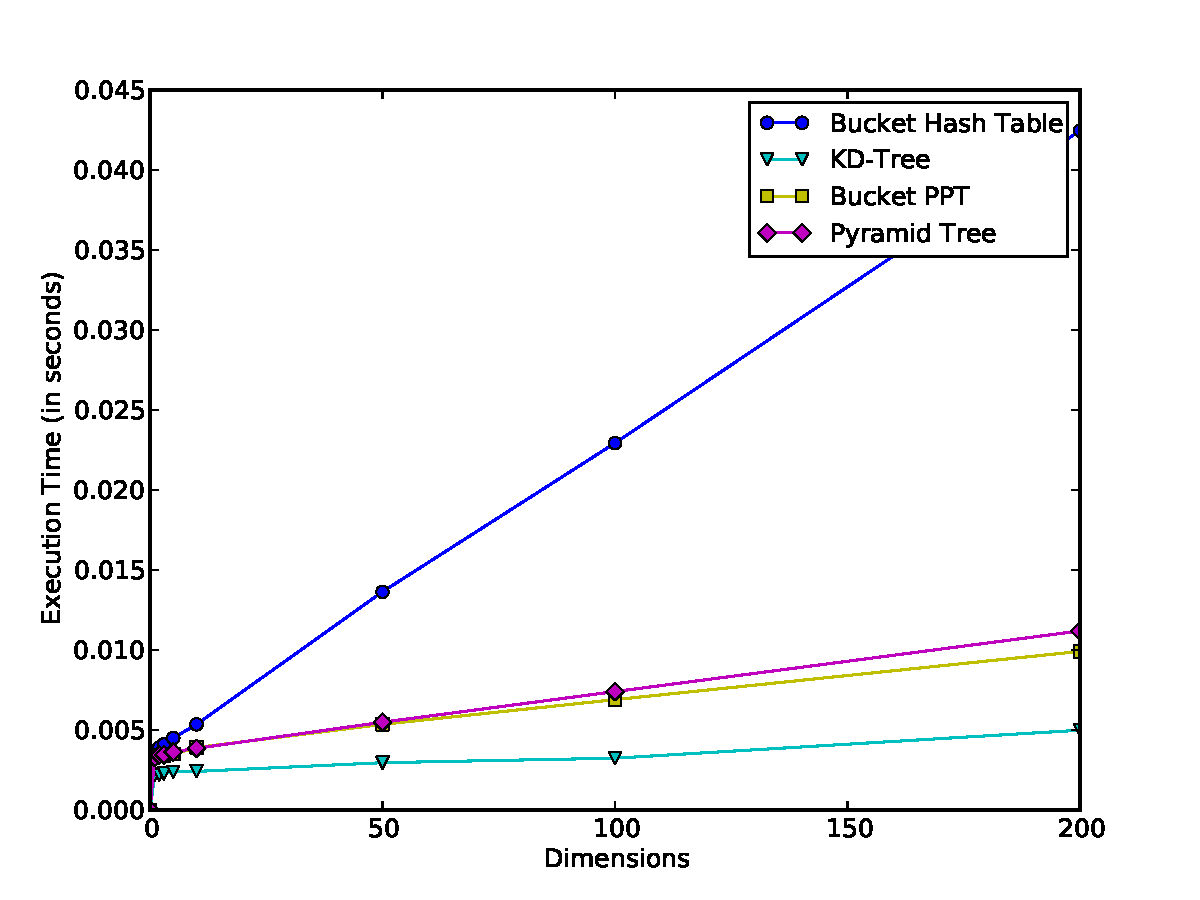
\includegraphics[scale=0.5]{figures/performance_analysis/iteration_3/randuniform_insert.pdf}
		}
		\end{subfloat}
		\begin{subfloat}[\texttt{delete}\label{fig:perf3-dimensionality-remove}]{%
			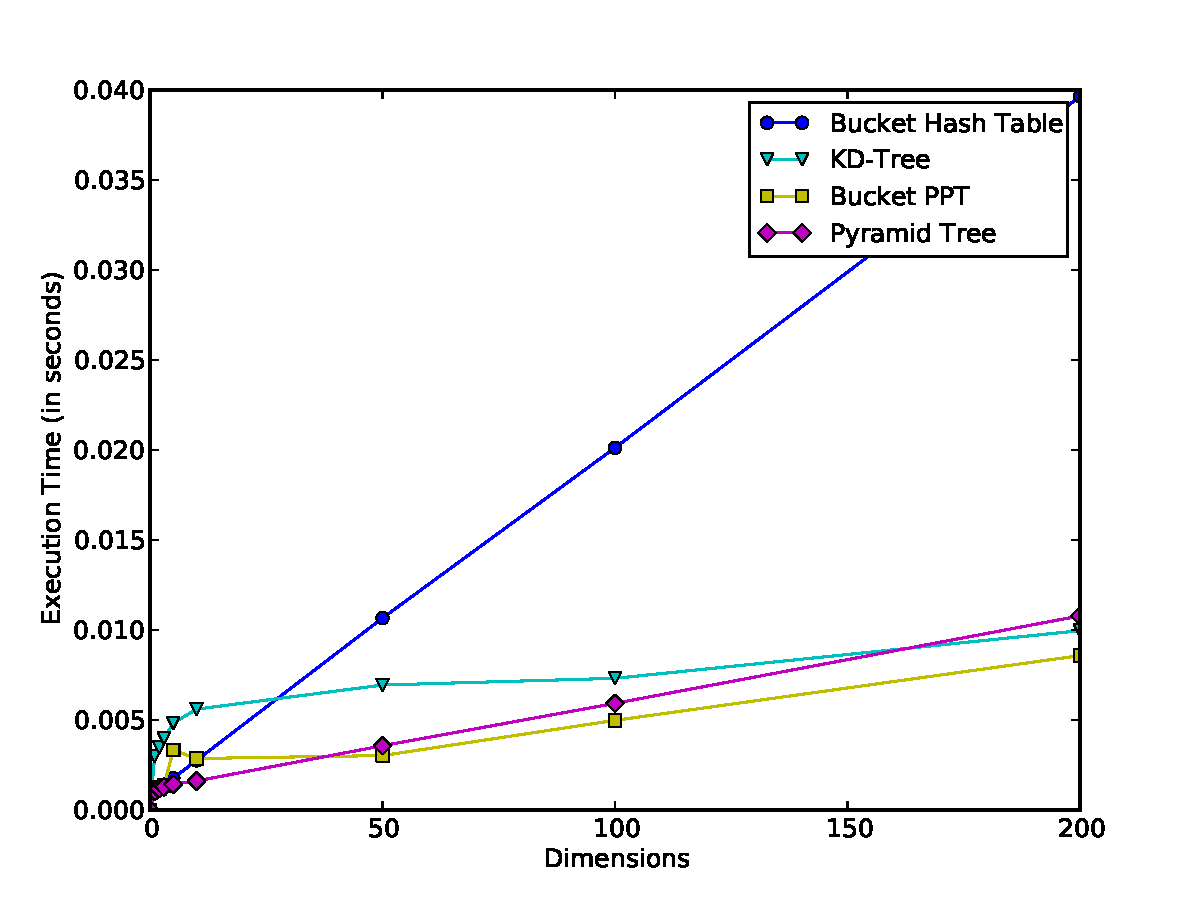
\includegraphics[scale=0.5]{figures/performance_analysis/iteration_3/randuniform_delete.pdf}
		}
		\end{subfloat}
	}%

	\caption{Index Structure Performance With Respect To Dimensionality (10,000 Points from Uniform Distribution Synthetic Dataset)}
	\label{fig:perf3-dimensionality}
\end{figure}

\begin{figure}
	\makebox[\textwidth][c]{%
		\begin{subfloat}[\texttt{insert}\label{fig:perf3-size-insert}]{%
			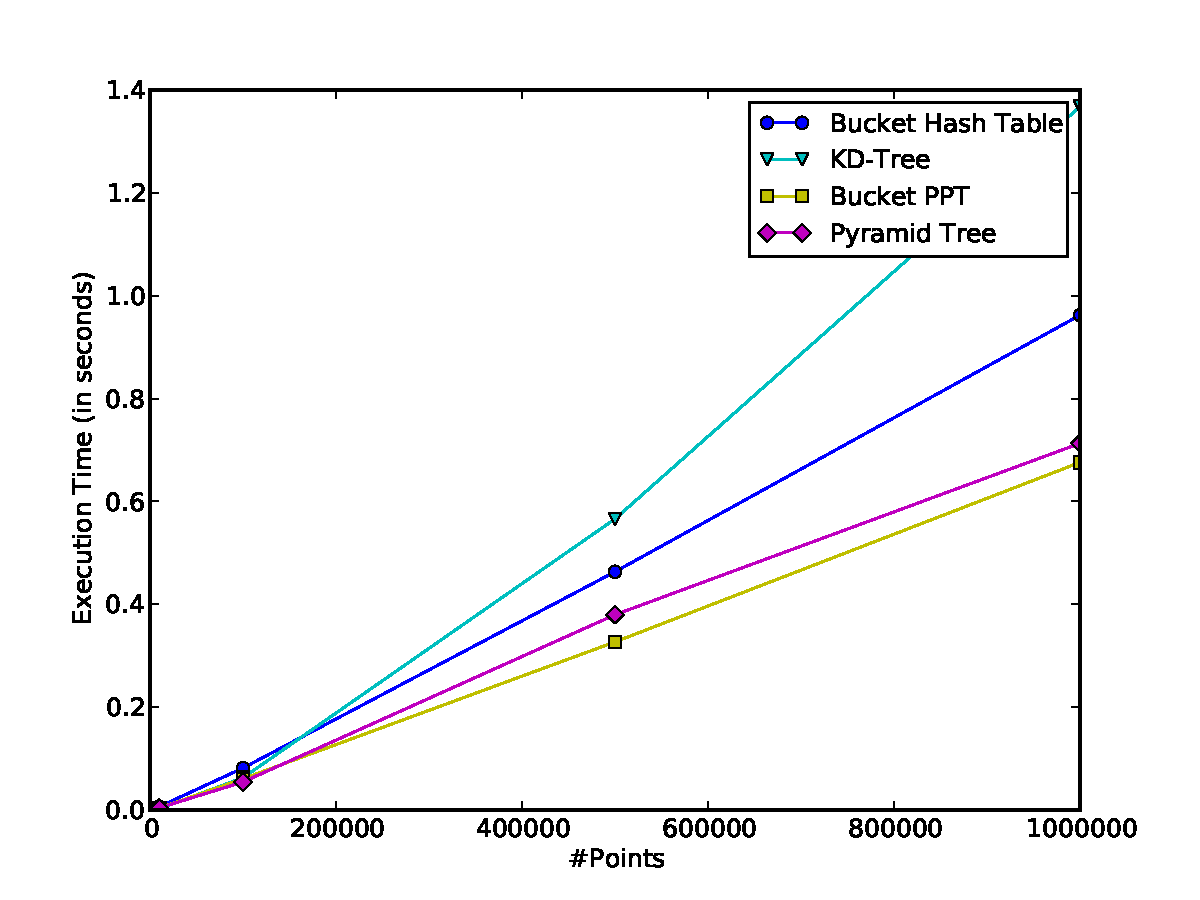
\includegraphics[scale=0.5]{figures/performance_analysis/iteration_3/sizevary_insert.pdf}
		}
		\end{subfloat}
		\begin{subfloat}[\texttt{delete}\label{fig:perf3-size-remove}]{%
			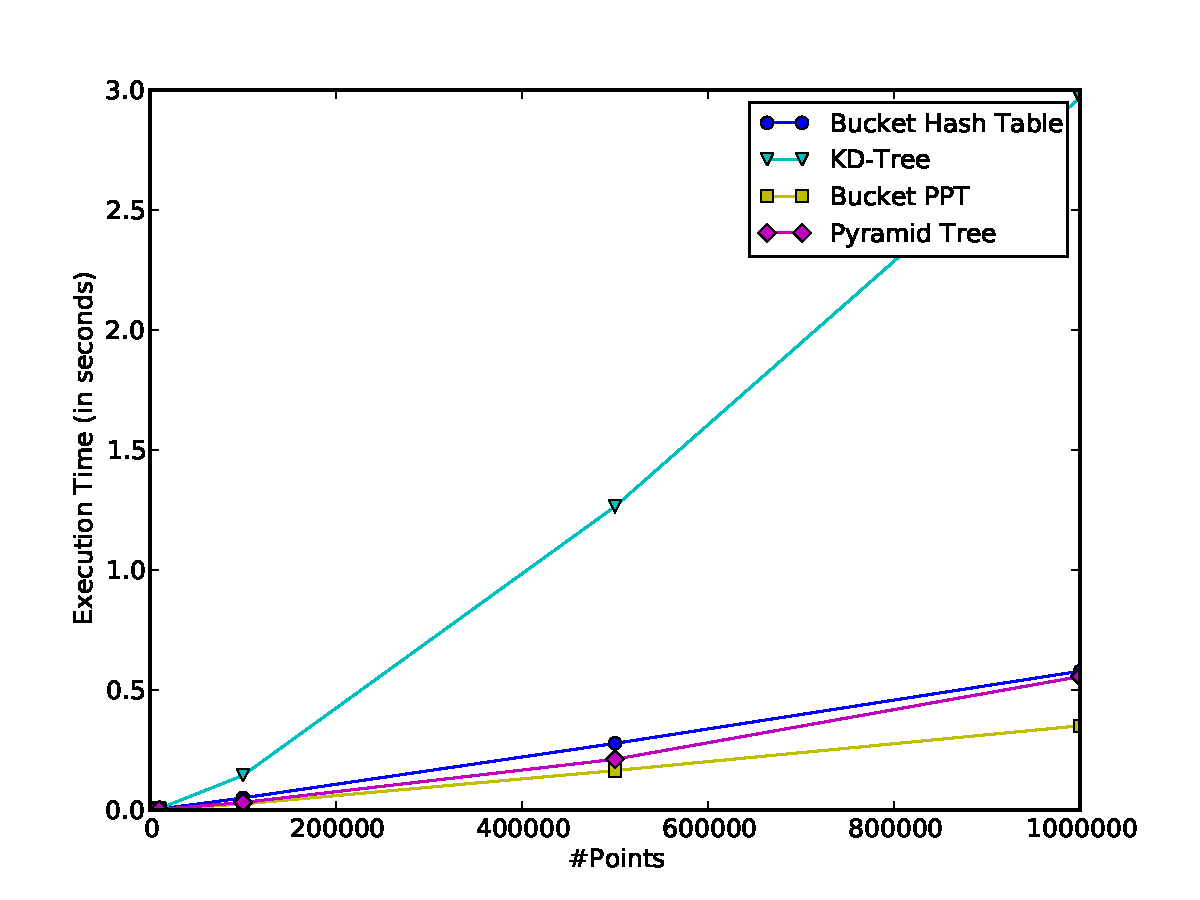
\includegraphics[scale=0.5]{figures/performance_analysis/iteration_3/sizevary_delete.pdf}
		}
		\end{subfloat}
	}%

	\caption{Index Structure Performance With Respect To Dataset Size (10,000 Points from Uniform Distribution Synthetic Dataset)}
	\label{fig:perf3-size}
\end{figure}

\begin{table}
	\centering
	\makebox[\textwidth][c]{%
		\begin{tabular}{|r|r|l|l|l|}
			\hline
			\multicolumn{2}{|c}{} & \multicolumn{3}{|c|}{\textbf{Dataset (Points)}} \\
			\hline
			\textbf{Structure} & \textbf{Operation} & \textbf{Astrophysics (500,000)} & \textbf{Hurricane Isabel (500,000)} & \textbf{Armadillo Mesh (435,544)} \\
			\hline
			\multirow{4}{*}{Bucket Hash Table} & Delete & 0.191339 & 0.248544 & 0.102674 \\
				& Insert & 0.360452 & 0.419106 & 0.2828 \\
				& Point Query & 0.172516 & 0.222288 & 0.0811833 \\
			\hline
			\multirow{4}{*}{$kd$-Tree} & Delete & 68.9612 & 578.798 & 0.91045 \\
				& Insert & 0.663231 & 0.434781 & 0.384241 \\
				& Point Query & 0.639265 & 0.408527 &  0.374425 \\
			\hline
			\multirow{4}{*}{Bucket PPT} & Delete & 82.908 & 71.006 & 0.160532 \\
				& Insert & 81.231 & 69.401 & 0.126938 \\
				& Point Query & 70.4391 & 69.3368 & 0.0956872 \\
			\hline
			\multirow{4}{*}{Pyramid Tree} & Delete & 33.7258 & 34.9182 & 0.164531 \\
				& Insert & 65.0126 & 69.5751 & 0.192165 \\
				& Point Query & 60.0216 & 69.4891 & 0.134481 \\
			\hline
		\end{tabular}
	}%
	\caption{Total Execution Time (in seconds) of Each Operation on Sampled Real Datasets}
	\label{tab:perf3-real}
\end{table}

\subsection{$kd$-Tree Balance}

The performance timings in the previous section show that the $kd$-tree becomes slower with particular datasets. Despite the $kd$-Tree storing the same number of points in each of the real datasets, the performance is different. The speed of processing 500,000 points from the astrophysics or hurricane Isabel datasets is much slower than the armadillo mesh or the synthetic datasets. 

The cause of this is most likely the \textit{balance} of the tree. Skewed datasets are known to affect the balance of spatial decomposition trees, resulting in longer paths from the root node to the leaves. To investigate this further, the \textit{balance factor} of the point $kd$-tree, when storing 500,000 points from three synthetic and three real datasets has been measured. The balance factor is defined as the \textit{average} length of a path from the root to a leaf. A lower balance factor means the $kd$-Tree has to visit less nodes on average when performing a point query, so queries will generally be faster. A $kd$-Tree is balanced when its balance factor is $\log_2 n$. When $n = 500,000$, the best possible balance factor is $\log_2 (500,000) \approx 19$. 

\begin{table}
	\centering
	\makebox[\textwidth][c]{%
		\begin{tabular}{|l|l|l|l|}
			\hline
			\textbf{Dataset} & \centrespecialcell{\textbf{Balance} \\ \textbf{Factor}} & \centrespecialcell{\textbf{Max Path} \\ \textbf{Length}} & \centrespecialcell{\textbf{Time to Query} \\ \textbf{All Points (seconds)}} \\
			\hline
			\leftspecialcell{Random 10D Points \\ (Uniform Distribution)} & 24.8285 & 47 & 0.591447 \\
			\leftspecialcell{Random 10D Points \\ (Skewed Distribution)} & 24.9092 & 44 & 0.602856 \\
			\leftspecialcell{Random 10D Points \\ (Clustered Distribution)} & 30.3362 & 57 & 0.479269 \\
			Astrophysics & 32.405 & 120 & 0.65575 \\
			Hurricane Isabel & 47.7236 & 123 & 0.466654 \\
			\hline
		\end{tabular}
	}%
	\caption{Point $kd$-Tree Balance Factor with 500,000 Points from Various Datasets}
	\label{tab:kdtree-balance-factor}
\end{table}

The balance factor clearly increases as $n$ is increased, so the concern here is how its affected by data distribution. Table \ref{tab:kdtree-balance-factor} contains the balance factor and maximum path length from the root to a leaf when the point $kd$-Tree is storing 500,000 points from different datasets. Here we see there appears to be little correlation between balance factor and query execution time. 

Despite the hurricane Isabel dataset introducing a higher balance factor and having three more dimensions than the astrophysics dataset, execution time 
so point comparisons take longer)

TODO: comment on results

\subsection{Summary}

This iteration showed that the point $kd$-tree, even with no attempts to further optimise the structure, significantly outperformed the Pseudo-Pyramid Tree and Pyramid Tree. The point $kd$-Tree is slightly slower than the Bucket Hash Table, but is more resilient to floating point inaccuracy as it does not rely on a potentially inaccurate hashing function. TODO: findings from skd-tree balance section